\section{Systematic Uncertainties}
\label{ch:Systematics}

\subsection{Spectra}
\label{sec:SystematicsSpectra}

Each contribution to the systematic uncertainty includes one or more variations that are considered for this analysis. The analysis is repeated from start to finish for each variation. The analysis uses ratios for each variation to the default solution for a given contribution and plots them together for review. Five contributions to the unfolding uncertainty are evaluated together in the same manner. For the majority of the contributions to the systematic uncertainty, the mean of the absolute value of the deviations to the default solution is determined for each \pT bin. For the contributions from unfolding, the maximum is used instead of the mean. In order to suppress nonphysical statistical fluctuations, most contributions are fitted with a polynomial, and the value of this fit at each bin center is taken as the true systematic uncertainty. Some contributions are evaluated without fitting, where the uncertainty is not expected to follow a clear pattern. All the uncertainties are then added in quadrature for each bin. All following contributions were considered for both \pp and \pPb collisions, unless otherwise stated. The section titles denote the uncertainties that were considered for only a single system.

\subsubsection{Tracking Efficiency}

The largest contribution to the systematic uncertainty at about 6--10$\%$ is the precision of the tracking efficiency, which is the probability of reconstructing a charged particle that passed through the detector, and primarily affects the scale of the spectrum. The uncertainty on the tracking efficiency was determined to be 4\% for the \pp dataset and 3\% for the \pPb dataset. The higher precision for the \pPb dataset is due to improved spacetime distortion corrections during run 2 as well as better performance of the ITS. The aforementioned "holes" in the SPD were not present during run 2. While the tracking efficiency uncertainty does change with momentum, most tracks within jets fall in a \pT range where the efficiency and the uncertainty on the efficiency are approximately constant~\cite{ALICE:2014sbx}. This quantity is varied by randomly discarding 4\% of Monte Carlo tracks in \pp and 3\% of Monte Carlo tracks in \pPb at detector level before jet finding and construction of the response matrix.

\subsubsection{Unfolding}

The second largest contribution arises from the combined unfolding uncertainties. This contribution is about 2--3$\%$ in \pp and about 5$\%$ for the majority of \pPb, other than where the transition between triggers occurs. These contributions primarily affect the shape of the spectrum. These contributions are as follows: 

\begin{itemize}
    \item[1)] The number of unfolding iterations is varied with +3/-2 iterations of Bayesian unfolding considered.
    \item[2)] The measured distribution and the response matrix are truncated at different values. The default minimum accepted jet \pT is 10 GeV. As variations, $\pm 5$ GeV are considered.
    \item[3)] The default prior is PYTHIA 8, the Monte Carlo used in the generation of the response. The ratio between the default unfolded solution and the default prior is applied as a weight to the original response matrix as a variation to the prior.
    \item[4)] The way in which the spectrum is binned at detector level causes statistically significant variations in the spectrum from unfolding. To ensure the final spectrum is not highly dependent on the way it is binned, four variations to the binning of the spectrum before unfolding are considered.
    \item[5)] Bayesian unfolding is used by default with SVD as a variation. The difference between the Bayesian and the SVD method is primarily used in order to account for the discrepancy seen between the two methods in the region where the triggers swap.
\end{itemize}

\subsubsection{EMCal Seed and Cell Thresholds}

The EMCal seed threshold is the lowest energy required for a signal in the EMCal to be considered for clusterization. The clusterization process adds all adjacent cells that are above the cell threshold to the cluster. The variations to the seed and cell thresholds are found in Table~\ref{tab:SeedCellThresholds}.


\begin{table}[hbt!]
    \centering
    \caption{Seed and cell threshold systematic variations for EMCal clustering.}
    \begin{tabular}{ | m{1.7cm} | m{4.1cm}| m{4.1cm} | } 
      \hline
      Variation & Seed Threshold (MeV) & Cell Threshold (MeV) \\
      \hline
      Default & 300 & 100 \\ 
      \hline
      Low & 275 & 75 \\ 
      \hline
      High & 350 & 100 \\ 
      \hline
    \end{tabular}
    \label{tab:SeedCellThresholds}
\end{table}

\subsubsection{Clusterizer Algorithm}

The default clusterizer algorithm used to cluster towers that pass the seed and cell thresholds in the EMCal is the "Clusterizer v3" algorithm. The NxN clusterizer with N = 3 and N = 5 are considered as variations, where N is the number of EMCal towers.

\subsubsection{Hadronic Correction}

The energy of clusters in the EMCal is corrected for the hadronic contribution. Since tracks are used in the analysis, the contribution from hadrons which leave deposits in the calorimeter must be subtracted off to avoid double counting the energy. By default, the momentum of the track in the ITS+TPC is fully subtracted from the cluster. While standard for jet analyses in ALICE, this is an extreme assumption, presuming that all tracks are electrons. The EMCal is not designed to measure the full hadronic energy due to its short hadronic interaction length, so hadrons interacting with the calorimeter material only leave partial showers. For this reason, the full subtraction of all tracks may lead to an over-correction for the hadronic energy. Two variations are considered. In one case, 70\% of the momentum of the matched tracks is subtracted. In the other, the minimally ionizing particle (MIP) energy is subtracted, which is 235.6 MeV in data and 282.4 MeV in Monte Carlo.

\subsubsection{Trigger Rejection Factor (\pp only)}

In \pp collisions, the trigger rejection factor is used to correct the downscaling of the spectra from different triggers. The rejection factor is calculated by linearly fitting to the ratio of triggers at the plateau after the turn-on. The cluster spectra are corrected for the cluster trigger efficiency. By default, this fit starts at 4 GeV for the lower trigger and 12.25 GeV for the higher trigger. Variations of $\pm 0.5$ GeV are considered. To account for the uncertainty on the rejection factor, the uncertainty extracted from these variations is combined with the uncertainty of the fit.

\subsubsection{Trigger Transition Threshold}

In order to combine the spectra from different triggers, a transition must occur from one trigger to the next once the higher threshold trigger reaches maximum efficiency. By default, the transition from the INT7 trigger to the EMC7 trigger in \pp collisions occurs at 30 GeV/$c$ of jet momentum, and the transition from the EMC7 trigger to the EJE trigger occurs at 60 GeV/$c$. In \pPb collisions, the transition from the INT7 trigger to the EJ2 trigger again occurs at 30 GeV/$c$, while the transition from the EJ2 trigger to the EJ1 trigger occurs at 60 GeV/$c$. Variations of $\pm 5$ GeV are considered for the transition to the lower threshold EMCal trigger, while variations of $\pm 10$ GeV are considered for the transition to the higher threshold EMCal trigger. The largest influences on this variation arise from the limited statistics of the lower threshold trigger with increasing \pT and the decreasing efficiency of the higher threshold trigger with decreasing \pT.

\subsubsection{Maximum Track Momentum and Cluster Energy}

An upper limit is placed on both the track momentum and cluster energy of 200 GeV by default. In this regime, the \pT resolution of charged tracks is significantly worse, so variations are required in order to reduce bias from tracks reconstructed with incorrect momentum. Variations of 125, 150, 175, and 225 GeV are tested. The selected upper range impacts the entire range of the spectra due to effects from unfolding.

\subsubsection{Q/\pT Shift}

The spectrum is varied for the Q/\pT shift caused by space-time distortions in the TPC. These distortions cause a momentum dependent offset in the number of positive and negative tracks which is studied by taking the ratio between the two. By default, no shift is considered. A 0.2$\%$ shift is considered as a variation. This shift was determined by running a PYTHIA8 simulation and applying a shift to the tracks. This analysis chooses the shift that is most closely aligned with data. Figure~\ref{fig:QoverPtShift} shows the comparison of different simulated Q/\pT shift values compared to ALICE data points in black. A linear fit to the simulated points is given for visual clarity.


\begin{figure}[hbt!]
    \centering
    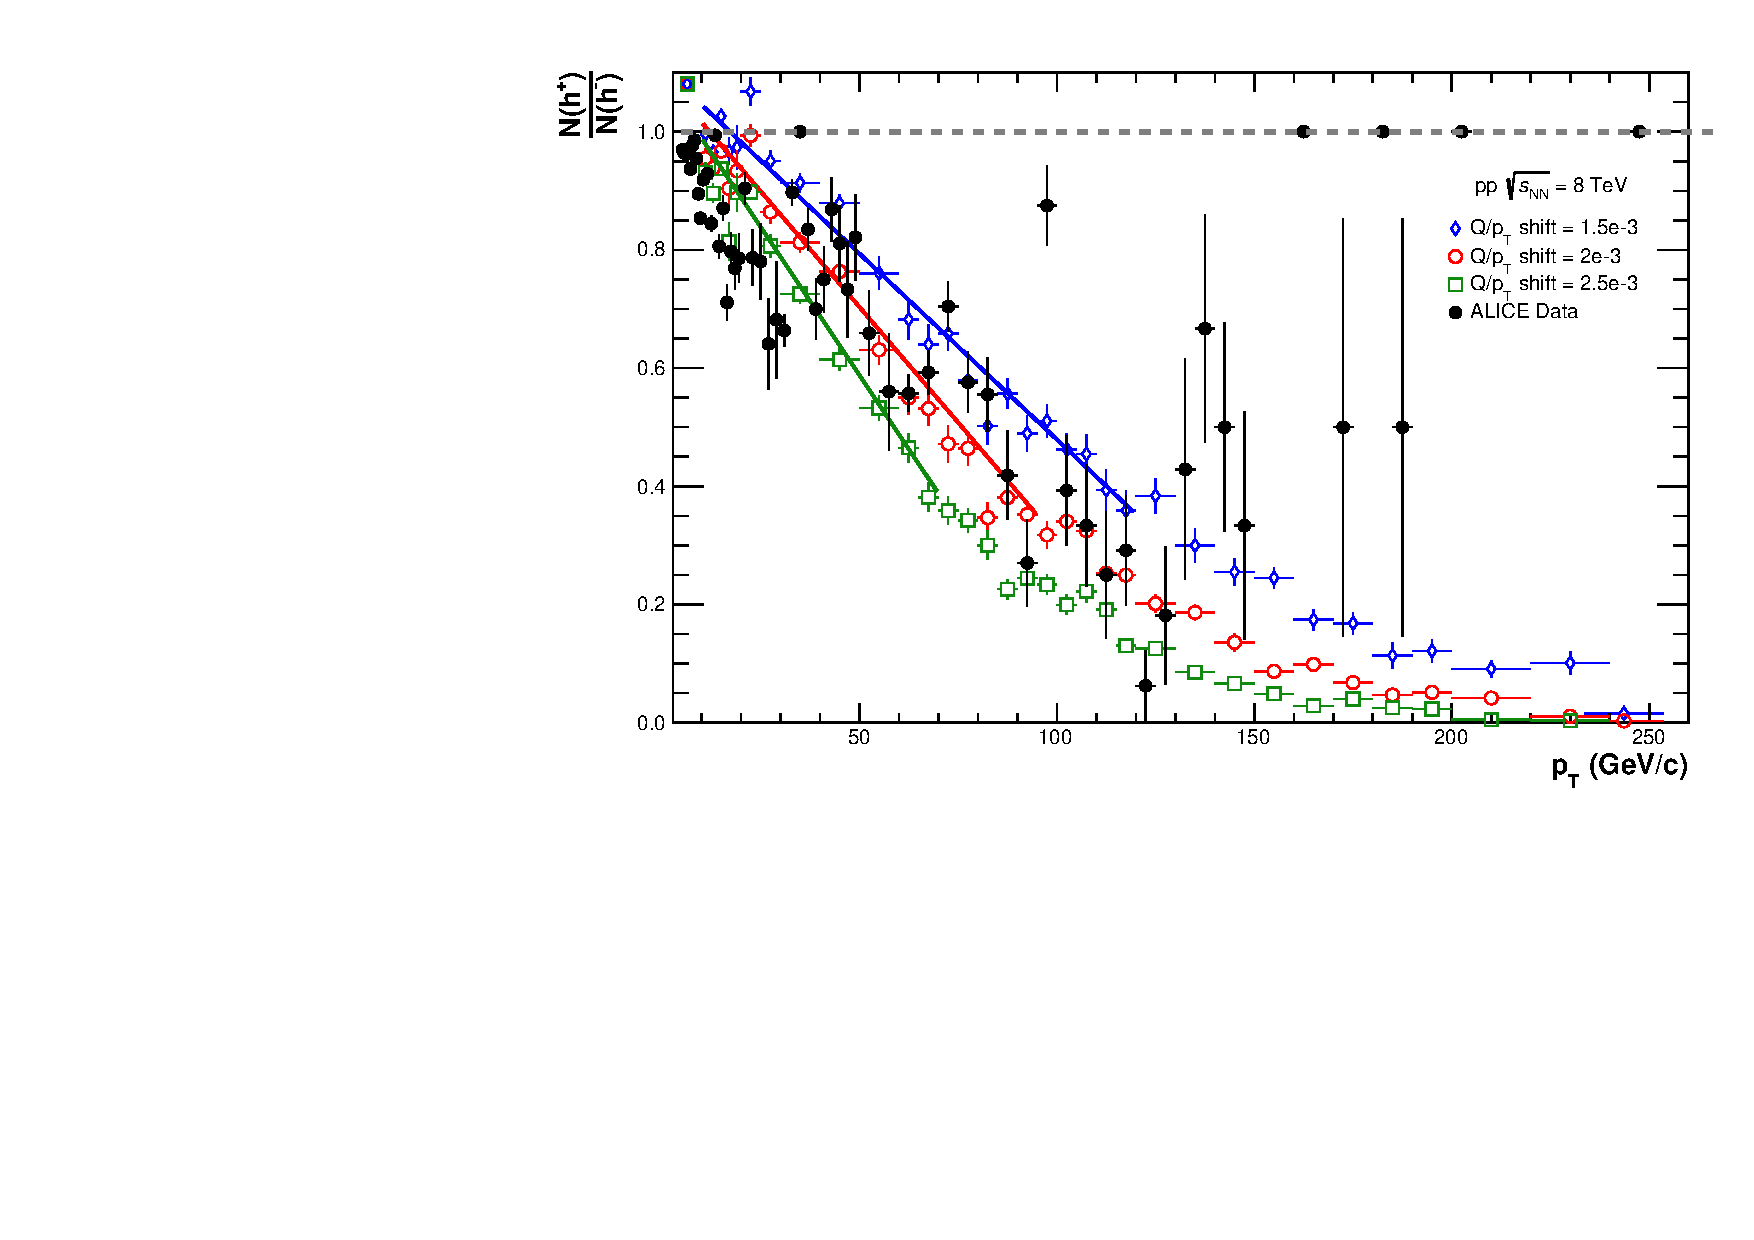
\includegraphics[width=15cm]{figures/QoverPtShift/QPTComparison.pdf}
    \caption{Comparison of different Q/\pT shift values showing the ratio of positive to negative tracks as a function of \pT. Three different simulated shift values are shown along with ALICE data.}
    \label{fig:QoverPtShift}
\end{figure}

\subsubsection{Background Fluctuations (\pPb only)}

Two additional uncertainties need to be considered for jets from \pPb collisions. The first one accounts for the uncertainty in the estimation of the background fluctuations around the average background density $\rho$. As discussed in Chapter~\ref{sec:backgroundSubtraction}, a $\delta$-\pT formed using the random cones method is used by default to smear the response matrix. As a variation, the $\delta$-\pT matrix is instead formed using single-track embedding. In this method, a track is embedded azimuthally perpendicular to the jet axis, where the underlying event is expected to dominate. The resulting momentum smearing is

\begin{equation}
    \delta \text{\pT}_\text{jet}^\text{emb} = \text{\pT}_\text{jet}^\text{raw,emb} - \rho_{\text{CMS}} A_\text{jet} - \text{\pT}^\text{emb}
\end{equation}

\noindent
where $\text{\pT}_\text{jet}^\text{raw,emb}$ is the reconstructed momentum of the jet with the embedded track, $A_\text{jet}$ is the jet area, $\rho_{\text{CMS}}$ is the estimated underlying event \pT density, and $\text{\pT}^\text{emb}$ is the transverse momentum of the embedded track.

\subsubsection{Luminosity (\pPb only)}

Downscaling the luminosity inspected by a trigger is a statistical process with finite precision. This process is needed because events are rejected for downscaling randomly, and there is a difference between the expected (configured) downscaling factor and the observed downscaling factor. In order to propagate the uncertainty on the luminosity into the spectrum, the luminosity is shifted by its corresponding uncertainty for EJ1 and EJ2 separately. The spectrum is scaled by this shifted luminosity, and the unfolded spectrum for each is taken as a variation.

\subsubsection{Total Systematic Uncertainty}

The components of the uncertainty are added in quadrature to obtain the total systematic uncertainty. Treating the uncertainties in this way assumes that they are uncorrelated. For an example, the different components of the systematic uncertainties for R = 0.2 jets in \pp collisions are shown in Figure~\ref{fig:SystematicsSpectraR02}. For other jet radii and individual contributions to the systematic uncertainty, see Appendix~\ref{sec:AppendixSystematics}. The equivalent plot for \pPb is shown in Figure~\ref{fig:SystematicsSpectraR02pPb}, and the equivalent Appendix is~\ref{sec:AppendixSystematicspPb}. In both cases, the uncertainty for nearly all contributions as well as the total systematic uncertainty grows with increasing \pT. The exceptions are the contributions from unfolding, trigger swap momentum variation, and luminosity scaling. These contributions to the uncertainty are largest in the momentum range where the transition between triggers occurs and the spectrum is most sensitive to the unfolding procedure. Other than in the \pT range where the triggers swap, the systematic uncertainty is comparable between the \pp and \pPb datasets with the lowest \pT point falling around 6--7\% uncertainty and the highest \pT point falling around 10--12\% uncertainty for $R$ = 0.2 jets. For both \pp and \pPb, the uncertainty grows with increasing jet resolution parameter, reaching approximately 10\% in the lowest \pT bins and approximately 14\% in the highest \pT bins for the largest jet radii studied. The uncertainties in the trigger transition region are more pronounced for \pPb collisions, reaching over 25\% for the largest radii studied.


\begin{figure}[hbt!]
    \centering
    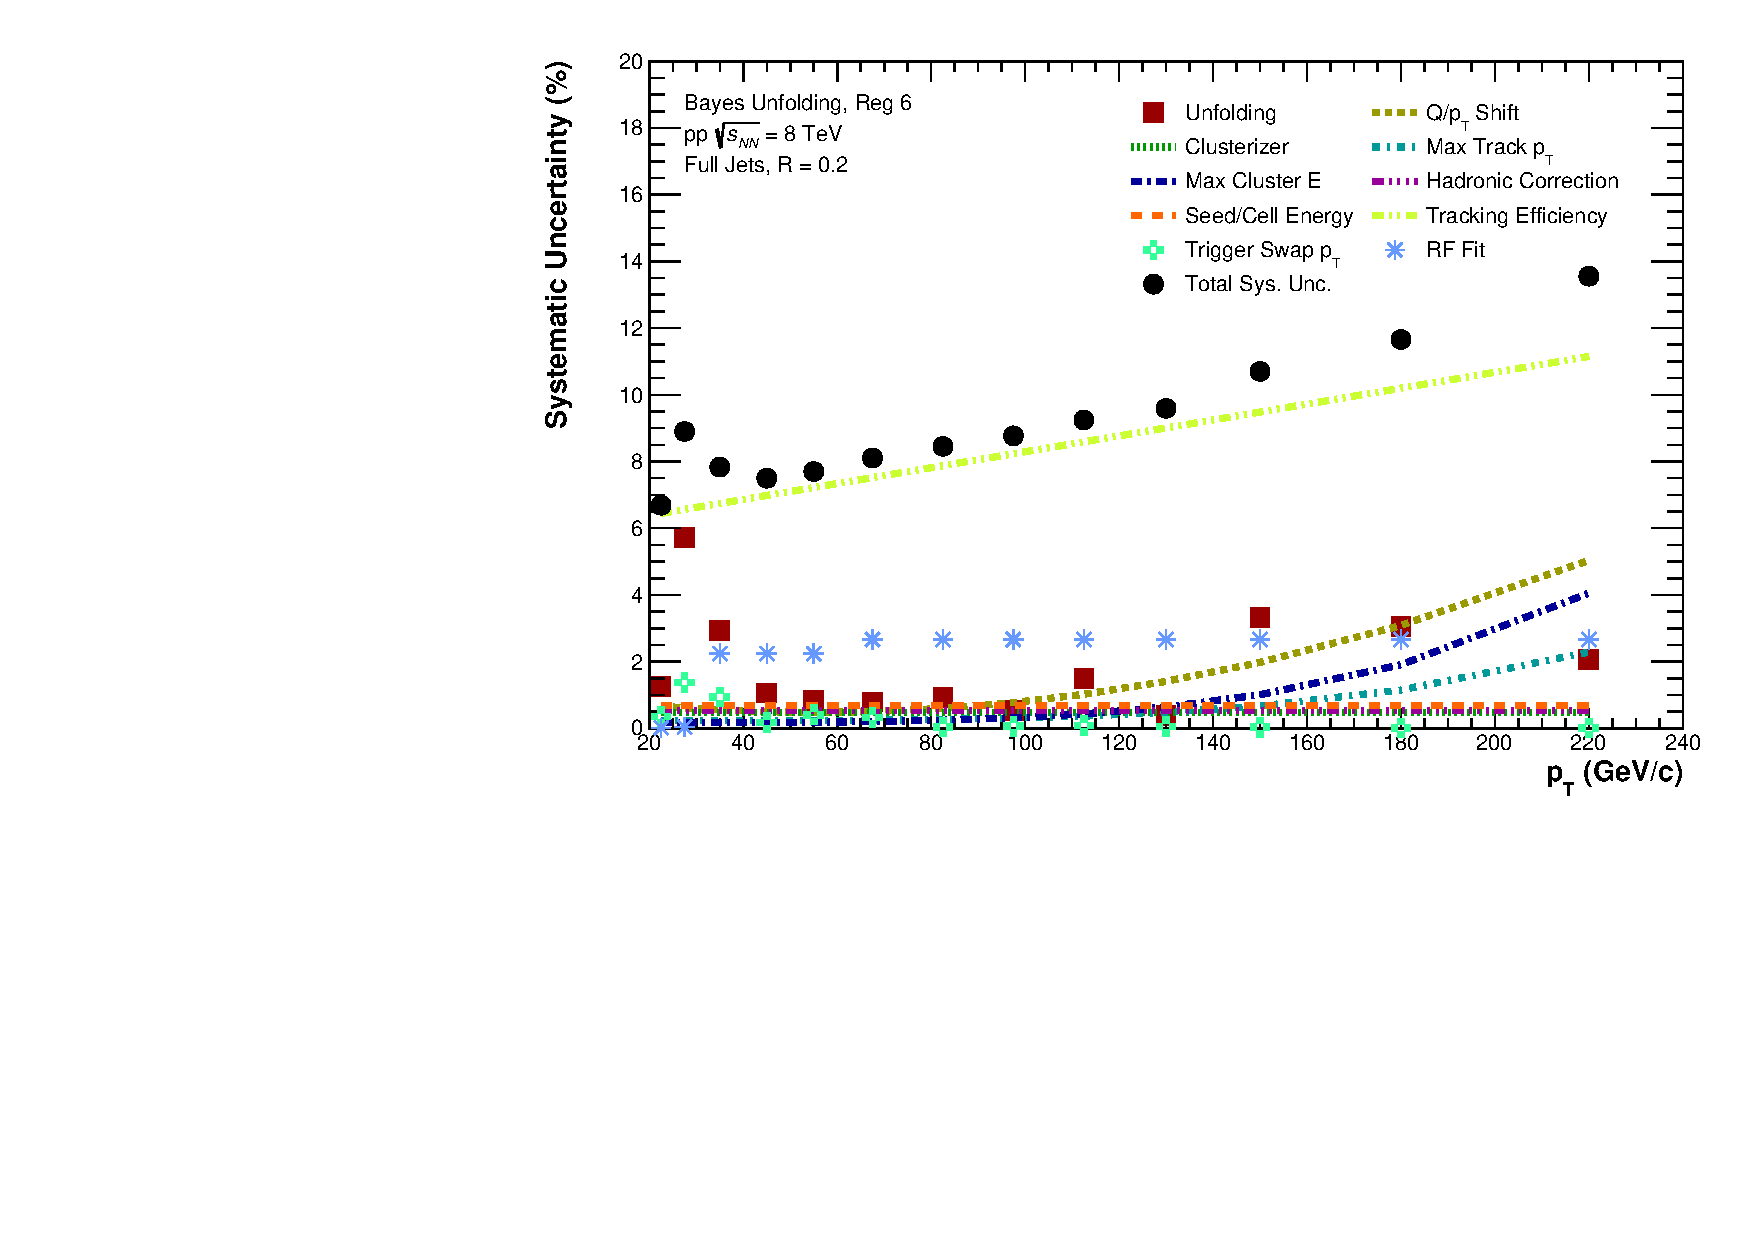
\includegraphics[width=15cm]{figures/Systematics/TotalSystematics_R02.pdf}
    \caption{All sources of systematic uncertainties in the jet spectrum, including the total systematic uncertainty with all components added in quadrature for $R$ = 0.2 jets in \pp collisions.}
    \label{fig:SystematicsSpectraR02}
\end{figure}

\begin{figure}[hbt!]
    \centering
    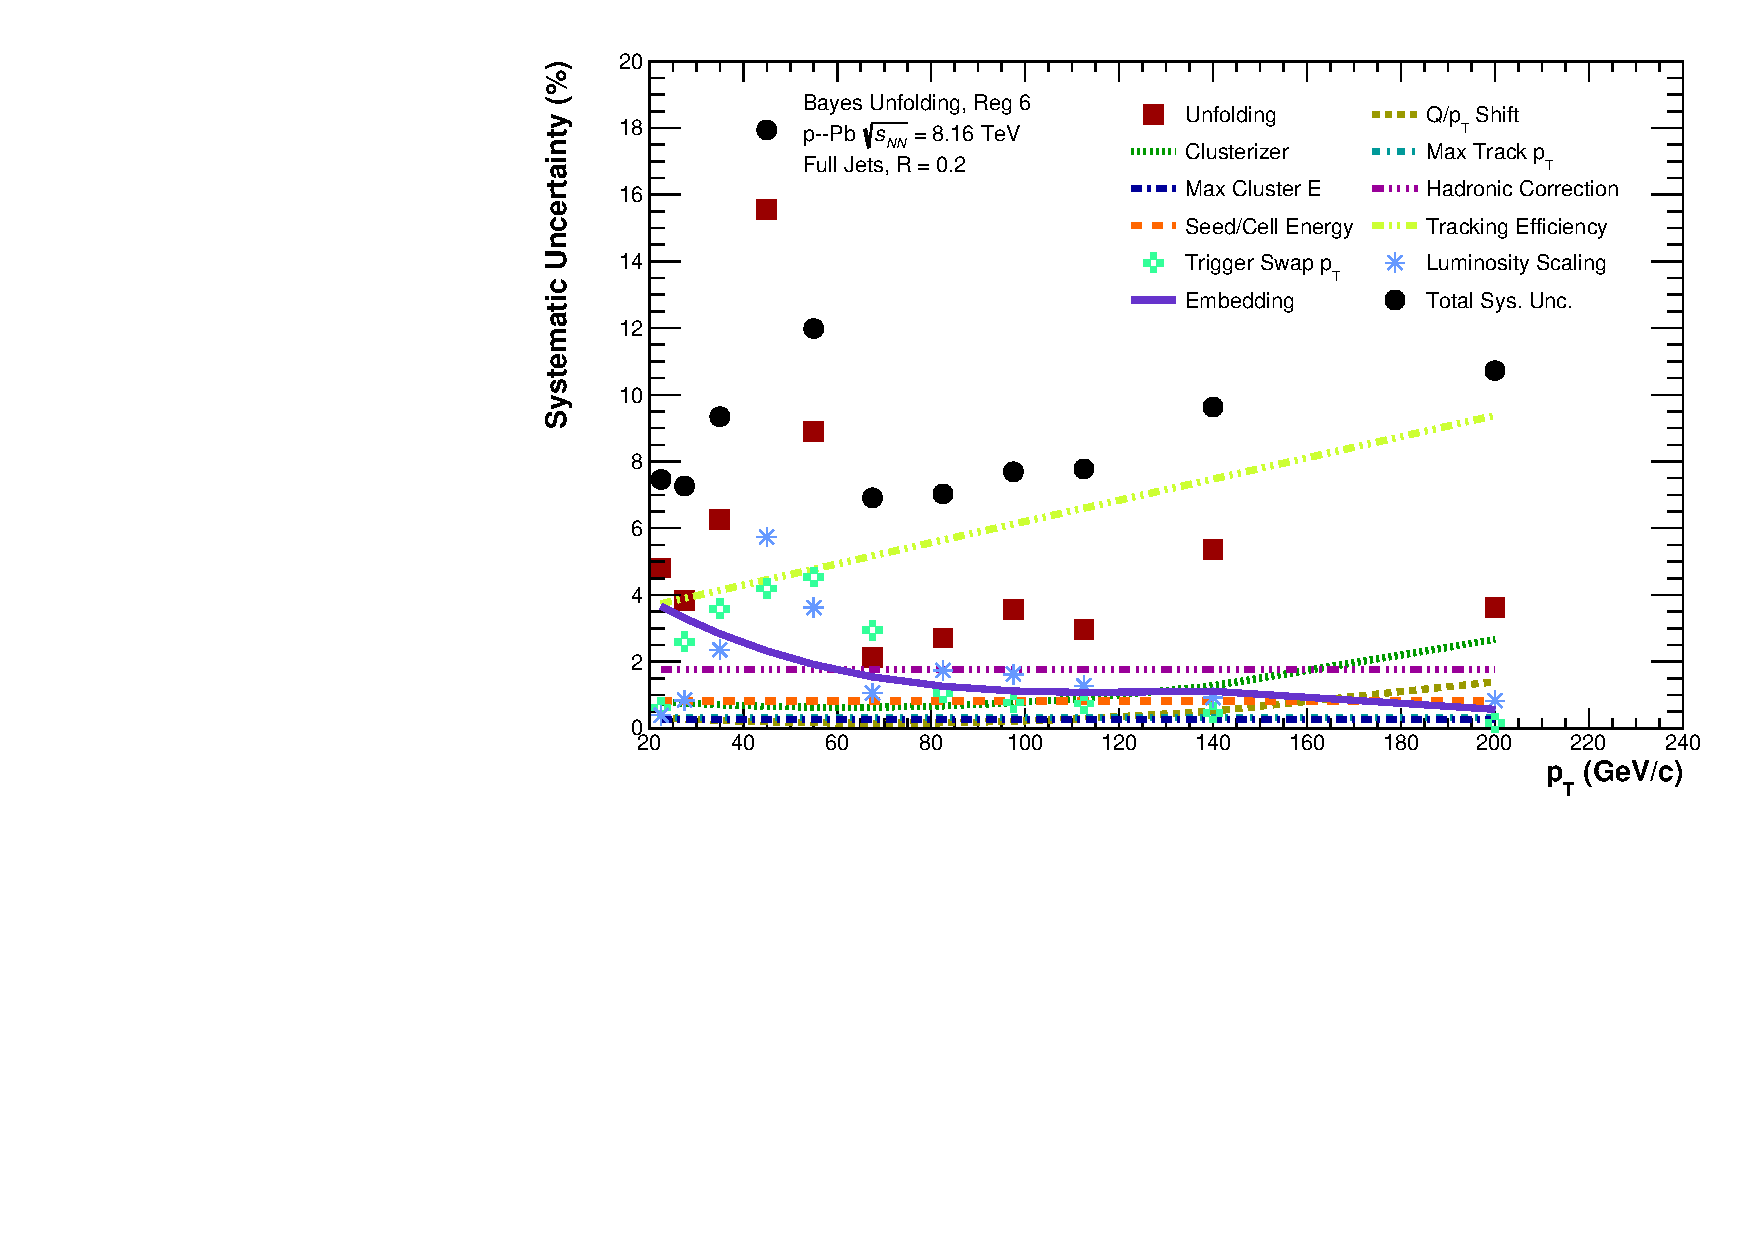
\includegraphics[width=15cm]{figures/pPbFigures/Systematics/TotalSystematics_R02.pdf}
    \caption{All sources of systematic uncertainties in the jet spectrum, including the total systematic uncertainty, with all components added in quadrature for $R$ = 0.2 jets in \pPb collisions.}
    \label{fig:SystematicsSpectraR02pPb}
\end{figure}

\subsection{Cross-Section Ratios}
\label{sec:SystematicsRatios}

For the cross-section ratios, the same systematic contributions are considered. With the exception of the trigger rejection factor fit, trigger swap, and unfolding systematic uncertainties, all contributions to the ratio are calculated directly resulting in partial cancellation. The rejection factor fit is not included at all since this contribution cancels entirely. The trigger transition and unfolding contributions for each cross-section in the ratio are added in quadrature to the total uncertainty. Figures~\ref{fig:SystematicsRatiosR02} and~\ref{fig:SystematicsRatiosR02pPb} give examples of the different components of the systematic uncertainties for R = 0.2/0.3 jets in \pp and \pPb collisions, respectively. For other jet radii and individual contributions, see Appendix~\ref{sec:AppendixSystematics} and~\ref{sec:AppendixSystematicspPb} for \pp and \pPb, respectively. In \pp collisions, the same trend is observed with the cross-section ratios. The systematic uncertainty grows with increasing jet \pT and jet resolution parameter. In \pPb collisions, the effect of the error treatment on the unfolding uncertainties is more pronounced. While other contributions partially canceled, the unfolding uncertainty does not. This results in a large uncertainty on the cross-section ratios in the trigger transition region. The larger uncertainty for \pPb collisions results from limited statistics where the INT7 trigger swaps to the EJ2 trigger. In this region, there is minimal overlap where the INT7 trigger runs out of statistics and the EJ2 trigger reaches maximum efficiency.


\begin{figure}[hbt!]
    \centering
    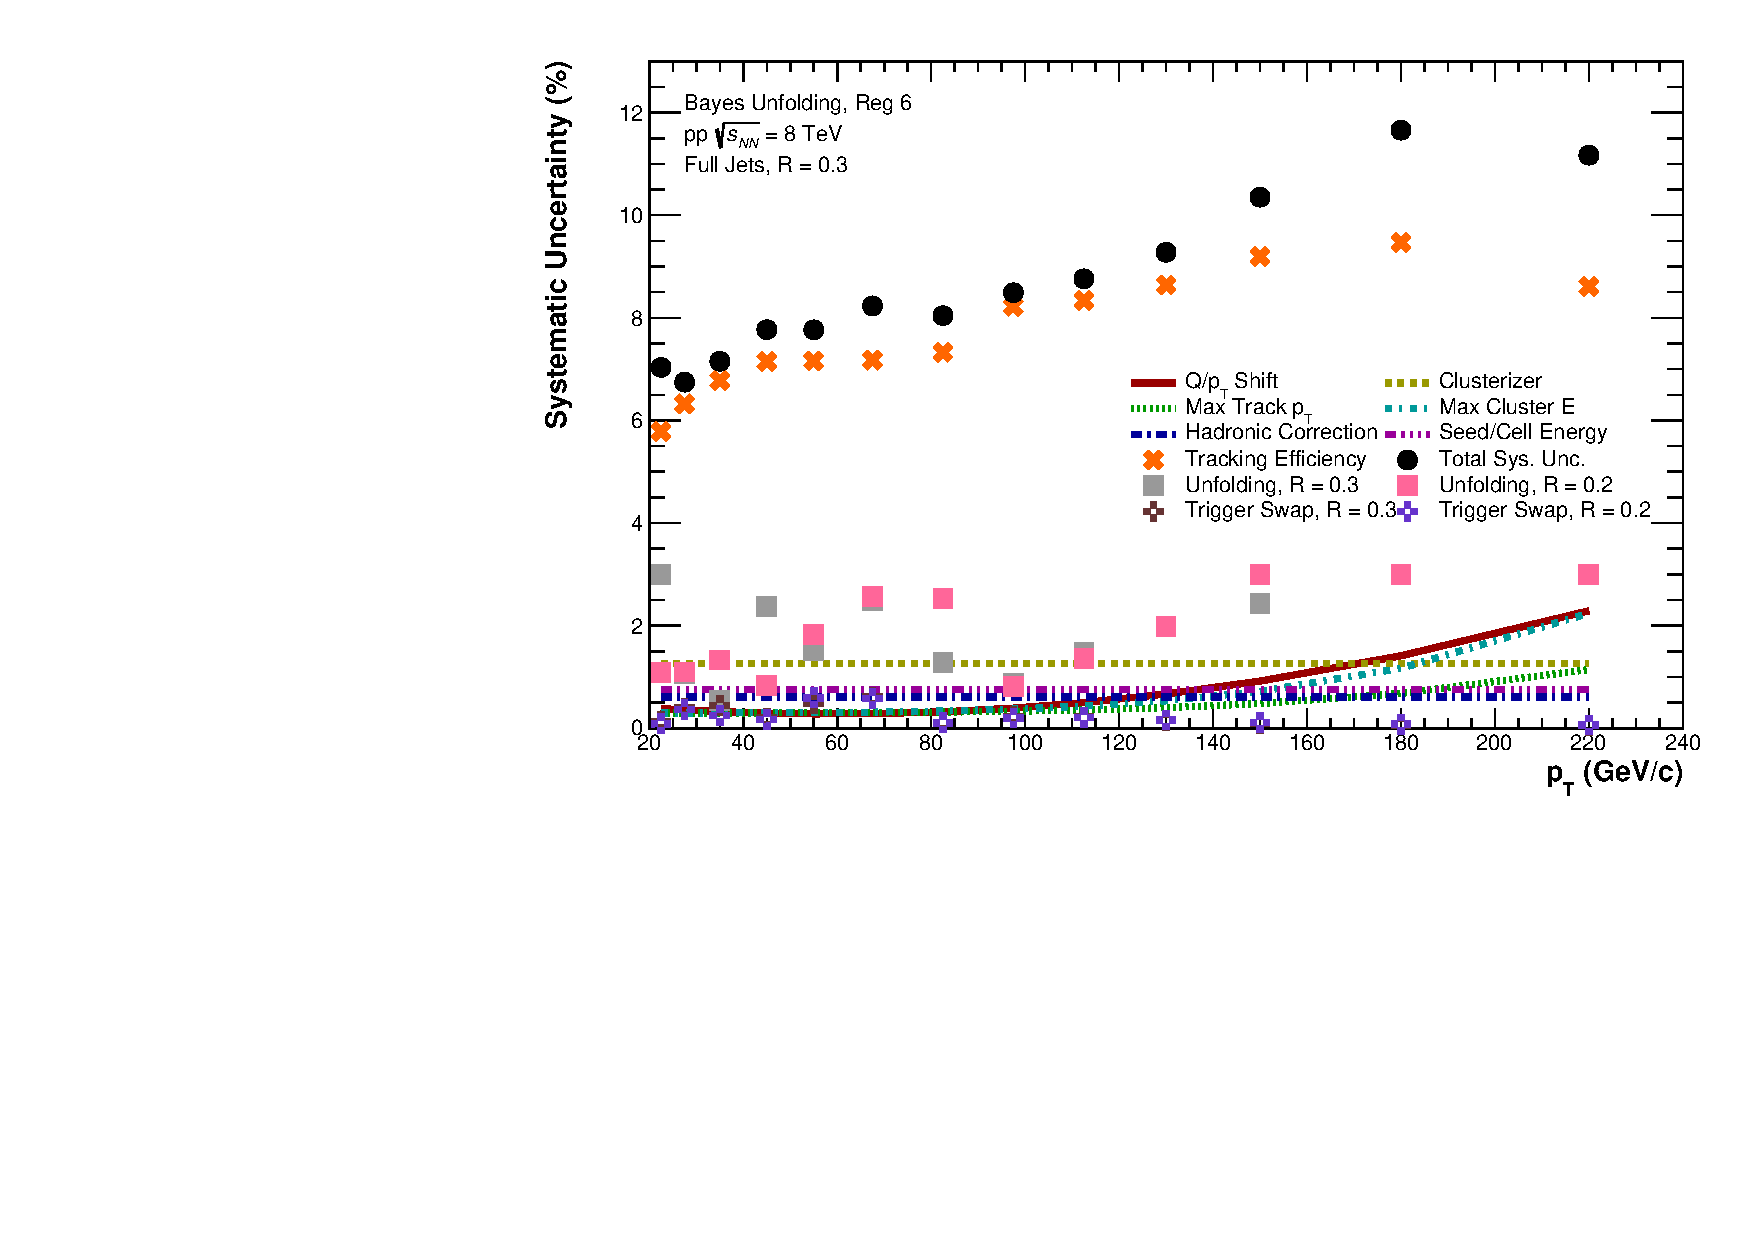
\includegraphics[width=15cm]{figures/Systematics/ratios/TotalSystematics_R02R03.pdf}
    \caption{All sources of systematic uncertainties in the cross-section ratio, including the total systematic uncertainty, with all components added in quadrature for $R$ = 0.2/0.3 jets in \pp collisions.}
    \label{fig:SystematicsRatiosR02}
\end{figure}

\begin{figure}[hbt!]
    \centering
    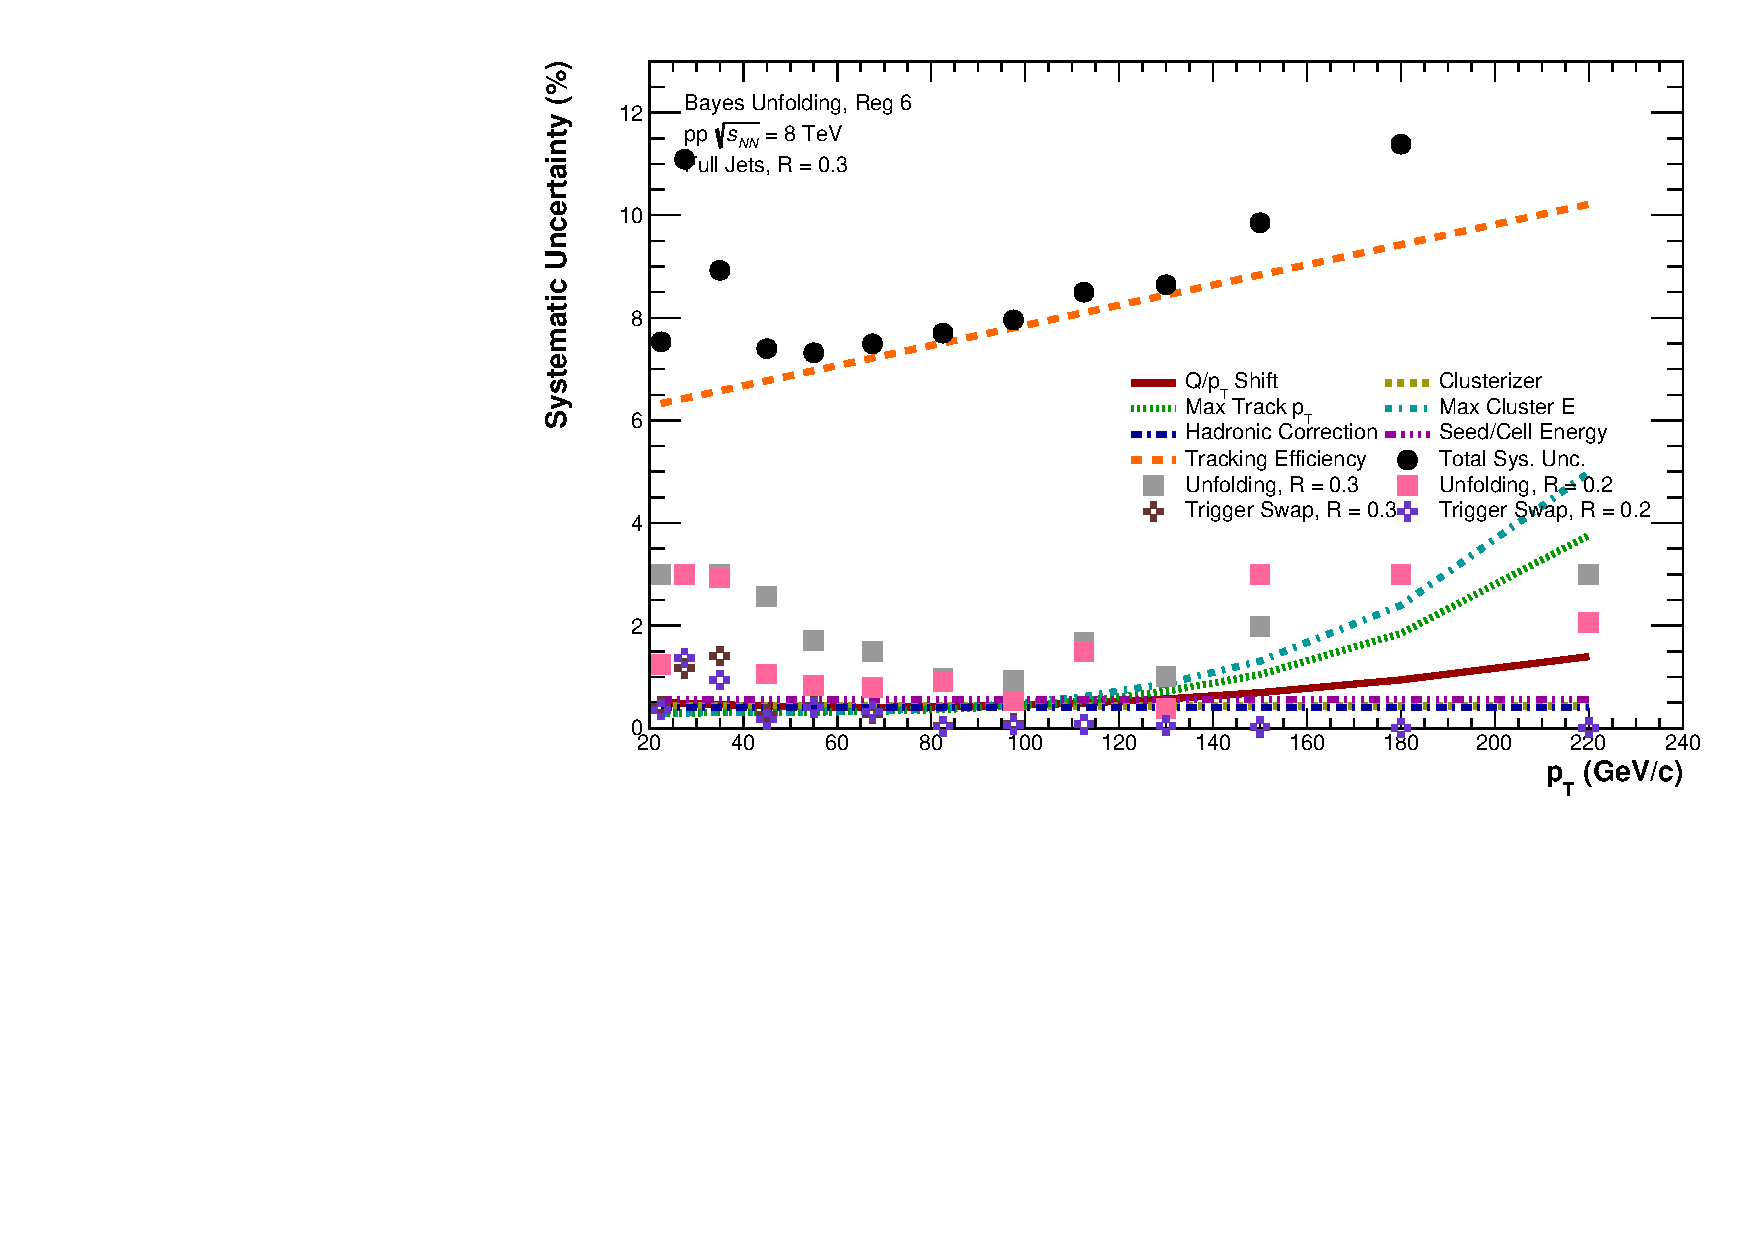
\includegraphics[width=15cm]{figures/pPbFigures/Systematics/ratios/TotalSystematics_R02R03.pdf}
    \caption{All sources of systematic uncertainties in the cross-section ratio, including the total systematic uncertainty, with all components added in quadrature for $R$ = 0.2/0.3 jets in \pPb collisions.}
    \label{fig:SystematicsRatiosR02pPb}
\end{figure}

\subsection{Nuclear Modification Factor}
\label{sec:systematicsRpA}

The uncertainties for the nuclear modification factor are handled in the same way as the cross-section ratios where the uncertainties are evaluated directly for the ratio and allow for error cancellation. The trigger rejection factor fit does not cancel, and the same is true for the luminosity. The trigger swap and unfolding contributions for each cross-section in the ratio are added in quadrature to the total uncertainty. The uncertainty from background fluctuations is also added in quadrature. The different components of the systematic uncertainties for R = 0.2 jets are shown in Figure~\ref{fig:SystematicsRpPbR02}. For other radii, see Appendix~\ref{sec:AppendixSystematicsRpPb}. The uncertainty is largest in the trigger transition region where the INT7 trigger runs out of statistics before the EJ2 trigger reaches maximum efficiency. As with the jet cross-sections and ratios, the uncertainty grows with increasing jet \pT and jet resolution parameter on average and has a peak in the trigger swap region. For comparison, a summary table of the systematic uncertainties on the \RpPb for charged particle jets at \sNN = 5.02 TeV is given in Table~\ref{tab:chj_sys}. The uncertainties for charged particle jets are generally smaller than for fully reconstructed jets in part due to the additional uncertainties introduced by the EMCal.


%\begin{figure}[hbt!]
%    \centering
%    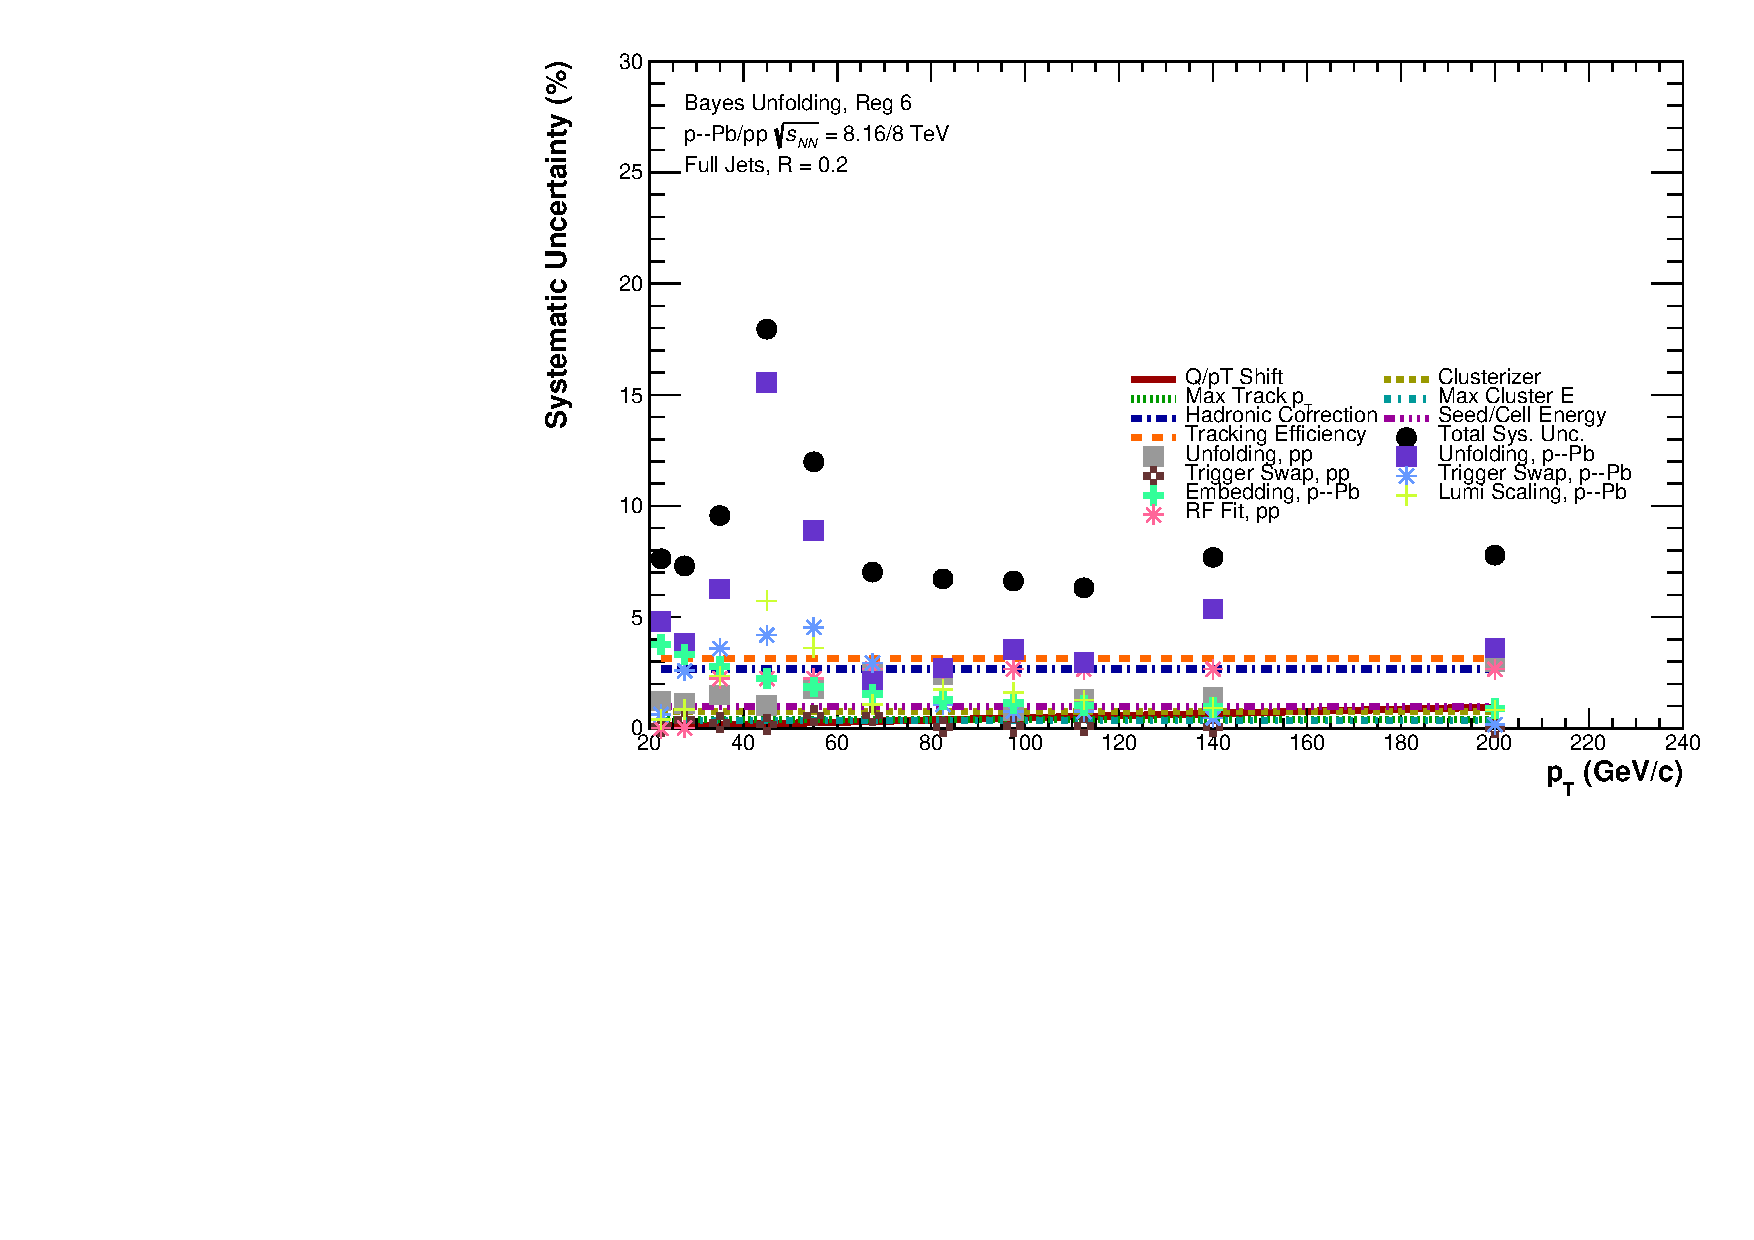
\includegraphics[width=15cm]{figures/pPbFigures/Systematics/RpPb/TotalSystematics_R02.pdf}
%    \caption{All sources of systematic uncertainties on the nuclear modification factor including the total systematic uncertainty with all components added in quadrature for $R$ = 0.2 jets.}
%    \label{fig:SystematicsRpPbR02}
%\end{figure}

\begin{table}[hbt!]
  \centering
  \caption{Summary of the systematic uncertainties for charged particle jets in \pp and \pPb collisions at 5.02 TeV~\cite{ALICE:2023ama}.}
  \begin{tabular}{  m{2.4cm}  m{4cm} m{4cm}  }
      \hline
      Radius & \pT Range (GeV/$c$) & Sys. Unc. (\%) \\
      \hline
      0.2 & 10--20 & 4.39 \\
          & 120--140 & 9.90 \\
      \hline
      0.3 & 10--20 & 4.83 \\
          & 120--140 & 11.23 \\
      \hline
      0.4 & 10--20 & 6.32 \\
          & 120--140 & 11.22 \\
      \hline
  \end{tabular}
  \label{tab:chj_sys}
\end{table}